\documentclass{beamer}
\usepackage[utf8]{inputenc}

\usetheme{Madrid}
\usecolortheme{default}
\usepackage{amsmath,amssymb,amsfonts,amsthm}
\usepackage{txfonts}
\usepackage{tkz-euclide}
\usepackage{listings}
\usepackage{adjustbox}
\usepackage{array}
\usepackage{tabularx}
\usepackage{gvv}
\usepackage{lmodern}
\usepackage{circuitikz}
\usepackage{tikz}
\usepackage{graphicx}
\usepackage{gensymb} % For using \degree symbol
\usepackage{enumitem}

\setbeamertemplate{page number in head/foot}[totalframenumber]

% Title Information
\title{4.13.8}
\date{October 9, 2025}
\author{ADHARVAN KSHATHRIYA BOMMAGANI - EE25BTECH11003}

\begin{document}

% Title Slide
\frame{\titlepage}

% Question Slide
\begin{frame}{Question}
The orthocentre of the triangle formed by the lines $x + y = 1$, $2x + 3y = 6$ and $4x - y + 4 = 0$ lies in the quadrant number.
\end{frame}

% Step 1: Given Lines
\begin{frame}{Theoretical Solution}
The three lines, written in the vector normal form $\mathbf{n}^\top \mathbf{x} = c$, are:
\begin{align}
     L_1: \myvec{1 \\ 1}^\top \myvec{x \\ y} = 1\\
     L_2: \myvec{2 \\ 3}^\top \myvec{x \\ y} = 6\\
     L_3: \myvec{4 \\ -1}^\top \myvec{x \\ y} = -4
     \end{align}
\bigskip
The vertices of the triangle, $\vec{A}$, $\vec{B}$, and $\vec{C}$, are the intersection points of these lines.
\end{frame}

% Step 2: Finding Vertices
\begin{frame}{Theoretical Solution}
    
         \textbf{Vertex A :} Solving $x+y=1$ and $2x+3y=6$.
        \begin{align}
            \myaugvec{2}{1 & 1 & 1 \\ 2 & 3 & 6}
            \xrightarrow{R_2 \to R_2 - 2R_1}
            \myaugvec{2}{1 & 1 & 1 \\ 0 & 1 & 4}
            \implies y=4, x=-3. \quad \vec{A}=\myvec{-3 \\ 4}
        \end{align}
        
       \textbf{Vertex B :} Solving $2x+3y=6$ and $4x-y=-4$.
        \begin{align}
            \myaugvec{2}{2 & 3 & 6 \\ 4 & -1 & -4}
            \xrightarrow{R_2 \to R_2 - 2R_1}
            \myaugvec{2}{2 & 3 & 6 \\ 0 & -7 & -16}
            \implies y=\frac{16}{7}, x=-\frac{3}{7} 
            \end{align}
            \begin{align}
            \vec{B}=\myvec{-3/7 \\ 16/7}
            \end{align}
   \end{frame}     
\begin{frame}{Theoretical Solution}
    

        \textbf{Vertex C :} Solving $x+y=1$ and $4x-y=-4$.
        \begin{align}
            \myaugvec{2}{1 & 1 & 1 \\ 4 & -1 & -4}
            \xrightarrow{R_2 \to R_2 - 4R_1}
            \myaugvec{2}{1 & 1 & 1 \\ 0 & -5 & -8}
            \implies y=\frac{8}{5}, x=-\frac{3}{5} 
          \end{align}  
            \begin{align}
            \vec{C}=\myvec{-3/5 \\ 8/5}
            \end{align}
            
        
    
\end{frame}
% Step 3: Equation of First Altitude
\begin{frame}{Theoretical Solution}
The altitude from $\vec{A}$ is perpendicular to the opposite side, which lies on line $L_3: 4x-y=-4$.
\begin{itemize}
    \item The direction of the altitude is parallel to the normal of $L_3$, which is $\myvec{4 \\ -1}$.
    \item The normal to the altitude is thus perpendicular to this direction, e.g., $\myvec{1 \\ 4}$.
\end{itemize}
\bigskip
So, the equation of the altitude is $x+4y=k$.
\bigskip
Since it passes through $\vec{A}=\myvec{-3 \\ 4}$:
\begin{align}
    (-3)+4(4)=k \implies k=13.
\end{align}
\textbf{Equation of Altitude AD}: $x+4y = 13$.
\end{frame}

% Step 4: Equation of Second Altitude
\begin{frame}{Theoretical Solution}
The altitude from $\vec{C}$ is perpendicular to the opposite side, which lies on line $L_2: 2x+3y=6$.
\begin{itemize}
    \item The direction of the altitude is parallel to the normal of $L_2$, which is $\myvec{2 \\ 3}$.
    \item The normal to the altitude is thus perpendicular to this direction, e.g., $\myvec{3 \\ -2}$.
\end{itemize}
\bigskip
So, the equation of the altitude is $3x-2y=k$.
\bigskip
Since it passes through $\vec{C}=\myvec{-3/5 \\ 8/5}$:
\begin{align}
    3(-\tfrac{3}{5})-2(\tfrac{8}{5})=k \implies k = -\frac{9}{5}-\frac{16}{5} = -5
\end{align}
\textbf{Equation of Altitude CE}: $3x-2y=-5$.
\end{frame}

% Step 5: Finding the Orthocentre
\begin{frame}{Theoretical Solution}
The orthocentre ($\vec{H}$) is the intersection of the altitudes. We solve the system:
\begin{align}
    x+4y&=13 \\
    3x-2y&=-5
\end{align}
Using Gaussian elimination:
\begin{align}
    \myaugvec{2}{
    1 & 4 & 13 \\
    3 & -2 & -5
    } \xrightarrow{R_2 \to R_2 - 3R_1}
    \myaugvec{2}{
    1 & 4 & 13 \\
    0 & -14 & -44
    }
\end{align}
\begin{itemize}
    \item From the second row: $-14y=-44 \implies y=\frac{22}{7}$.
    \item Substituting into the first row: $x+4(\tfrac{22}{7})=13 \implies x=\frac{3}{7}$.
\end{itemize}
\end{frame}

% Step 6: Final Answer
\begin{frame}{Theoretical Solution}
The coordinates of the orthocentre are:
\begin{align}
    \vec{H} = \myvec{\frac{3}{7} \\ \frac{22}{7}}
\end{align}
\bigskip
Since the x-coordinate ($\tfrac{3}{7}$) and the y-coordinate ($\tfrac{22}{7}$) are both positive, the orthocentre lies in the \textbf{first quadrant}.
\end{frame}

% Step 7: Figure
\begin{frame}{Plot}
\centering
\textbf{Plot of the Lines and Orthocentre:}
\begin{figure}[h!]
    \centering
    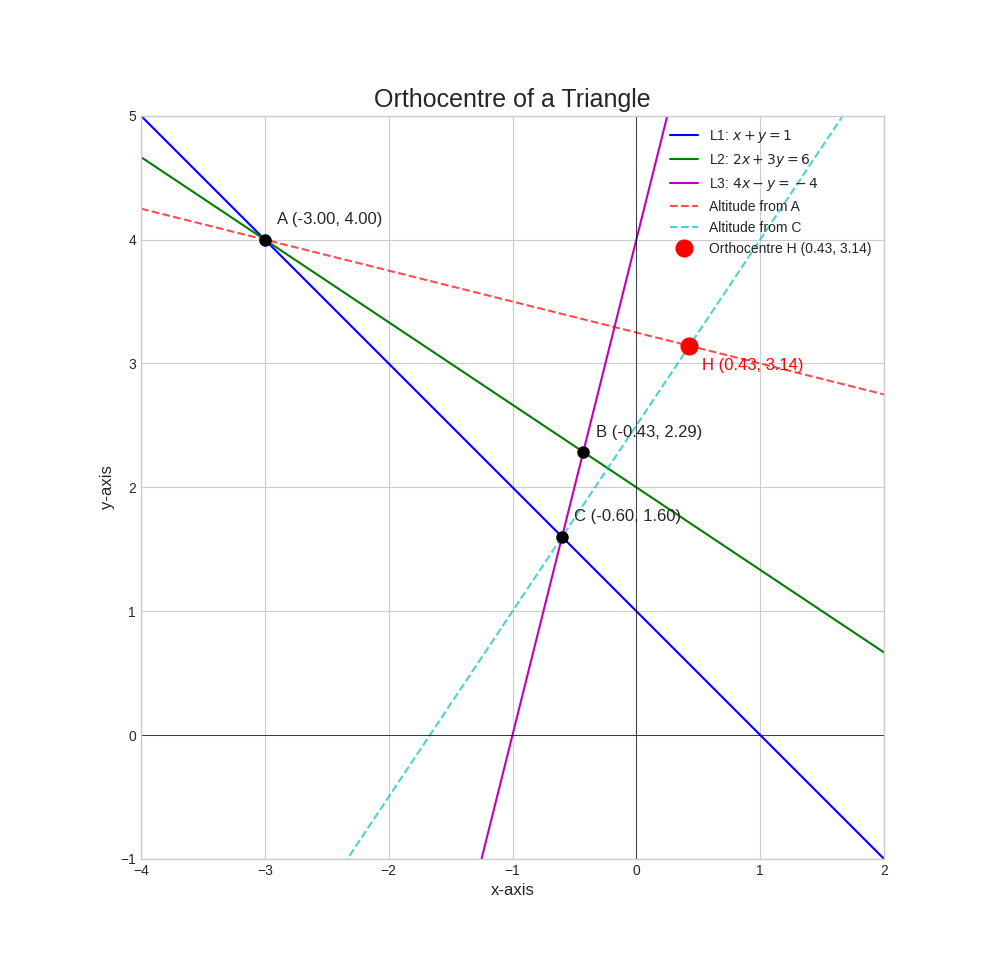
\includegraphics[width=0.7\columnwidth]{figs/fig1.png}
    \caption{The triangle (solid lines), its altitudes (dashed), and the orthocentre $\vec{H}$.}
\end{figure}
\end{frame}

\end{document}